% =========================================================================
% SECTION 3: ANDROID IMPLEMENTATION
% =========================================================================
\section{Android Implementation}
\label{sec:implementation}

\subsection{Camera Ingestion and Bounded Backpressure}
\label{sec:impl_camera}
\texttt{AndroidCameraFrameSource} connects to the rear camera using Jetpack CameraX \texttt{ImageAnalysis} targeting 30\,FPS. To prevent latency accumulation when CPU scheduling fluctuates, the analyzer operates under \texttt{STRATEGY\_KEEP\_ONLY\_LATEST} with a single-frame buffer ($N=1$). If the worker thread is busy, incoming frames are discarded immediately at the driver level rather than buffering in memory.

\texttt{FrameBackpressurePolicy} tracks frame delivery intervals. When an inter-frame interval exceeds $\Delta t > 0.25$\,s, the system switches to \texttt{DEGRADED} mode, falling back to static proximity rules. Negative intervals ($\Delta t < 0$) from clock adjustments command an immediate \texttt{EMERGENCY\_STOP}. To eliminate processing overhead, the analyzer reads the Y (luminance) plane directly from incoming \texttt{YUV\_420\_888} buffers, avoiding colorspace conversion and bitmap allocations. Native capture resolution is $640 \times 480$ pixels (measured at 24.9\,FPS on device).

\subsection{Spatial Perception and Candidate Extraction}
\label{sec:impl_perception}
\texttt{AndroidPerceptionAnalyzer} downsamples the luminance plane onto a $32 \times 24$ grid ($\Delta u = W/32, \Delta v = H/24$). This reduces per-frame evaluations from 307,200 pixels to 768 cells. For each cell $(r, c)$, horizontal and vertical Sobel gradient energies are computed:
\begin{equation}
E(r, c) = |I(r, c+1) - I(r, c-1)| + |I(r+1, c) - I(r-1, c)|
\label{eq:sobel_energy}
\end{equation}
Cells exceeding edge energy $E > 38.0f$ and local $3 \times 3$ contrast $> 24.0f$ below the optical horizon line ($v_{\text{horiz}} = c_y - f_y \tan\theta_p$) are marked active. Contiguous active cells are grouped into spatial clusters via 4-connectivity Breadth-First Search (BFS). Clusters smaller than 6 cells are dropped as noise. Surviving clusters are classified into morphology types: \texttt{COMPACT\_VOLUME}, \texttt{ELONGATED\_STRUCTURE}, \texttt{PLANAR\_FLOOR\_FEATURE}, or \texttt{UNCERTAIN}.

% Figure 3: Ground-Plane Projection Geometry with Pitch/Roll Compensation (Monochrome 300 DPI)
\begin{figure}[!t]
\centering
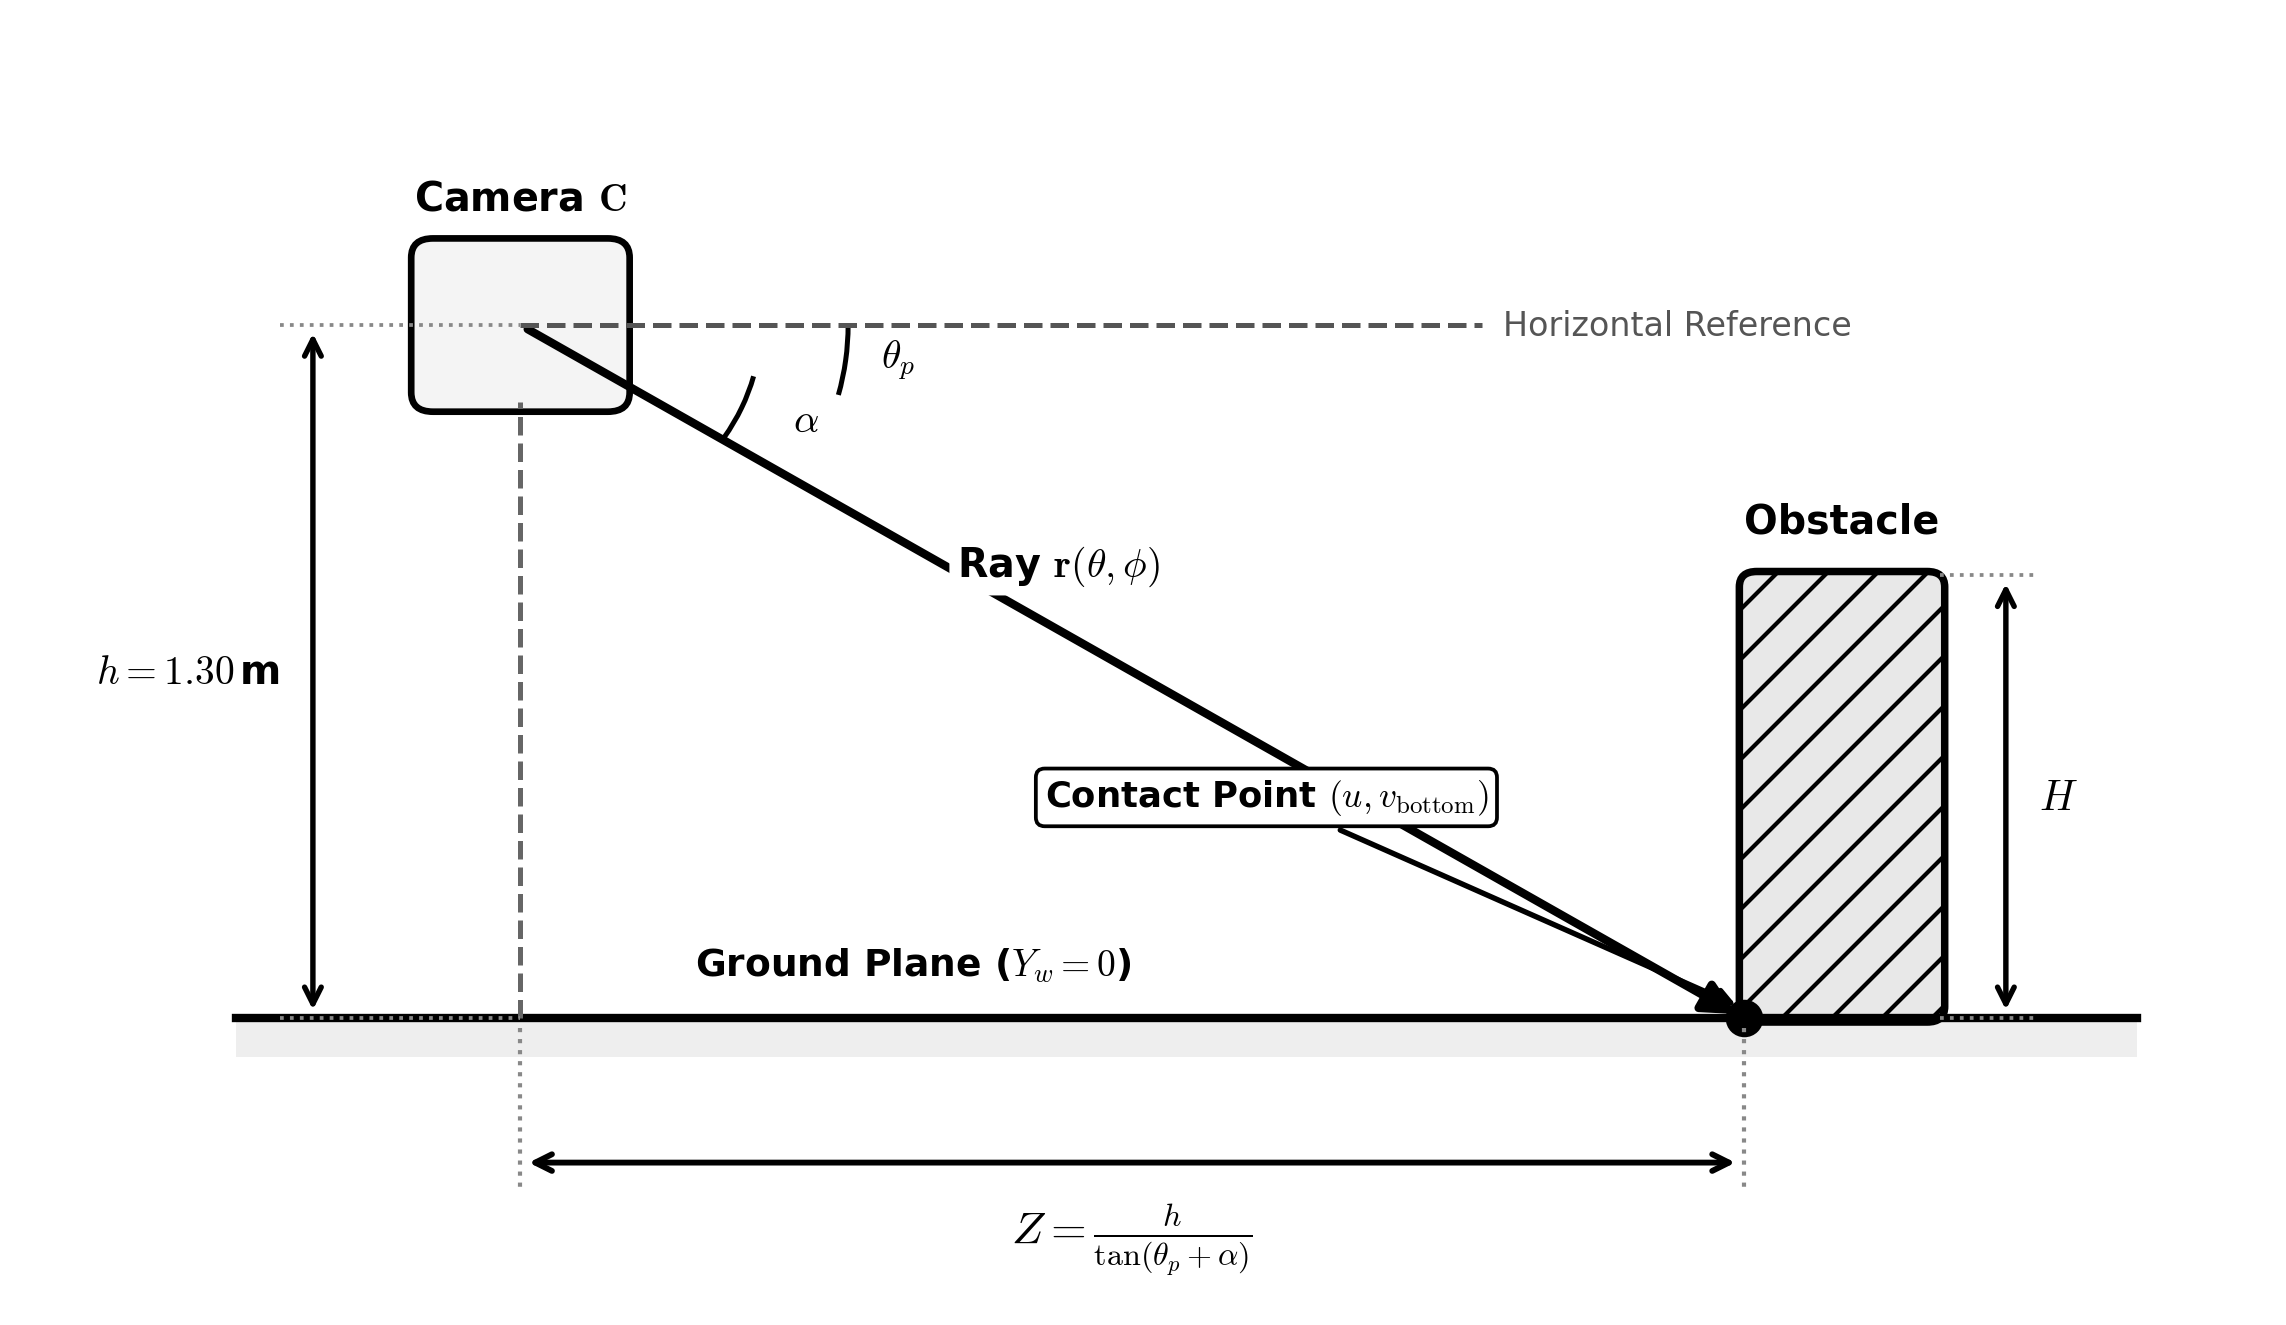
\includegraphics[width=\columnwidth]{figures/fig_projection.png}
\caption{Monocular ground-plane inverse ray projection geometry (black and white): bottom contact point $(u, v_{\text{bottom}})$ is projected onto ground plane $Y_w = 0$ incorporating IMU pitch $\theta_p$ and roll $\phi$ to recover metric distance $Z$, lateral offset $X$, and obstacle height $H$.}
\label{fig:ground_projection_geometry}
\end{figure}


\subsection{Geometric Validation and Ground Projection}
\label{sec:impl_geometry}
Given camera mount height $h = 1.30$\,m, mount pitch $\theta_p = 12^\circ$ ($0.209$\,rad), and intrinsics $(f_x, f_y, c_x, c_y)$~\cite{zhang2000flexible,hartley2003multiple}, candidate bottom contact pixels $(u, v_{\text{bottom}})$ are projected onto ground plane $Y_w = 0$ incorporating dynamic IMU pitch $\theta$ and roll $\phi$~\cite{criminisi2000single,cathey2005perspective} (Fig.~\ref{fig:ground_projection_geometry}):
\begin{align}
x_n &= \frac{u - c_x}{f_x}, \quad y_n = \frac{v_{\text{bottom}} - c_y}{f_y} \\
r_x &= x_n \cos\phi - y_n \sin\phi \label{eq:rx} \\
r_y &= (x_n \sin\phi + y_n \cos\phi) \cos\theta + \sin\theta \label{eq:ry} \\
r_z &= -(x_n \sin\phi + y_n \cos\phi) \sin\theta + \cos\theta \label{eq:rz}
\end{align}
The denominator $r_y$ represents the downward component of the optical ray. Rays with $r_y \le 0.04$ point near or above the horizon and are rejected as \texttt{INVALID\_GROUND\_RAY}. For valid rays, scale $t = h / r_y$ yields ground Cartesian coordinates:
\begin{equation}
Z = t \cdot r_z, \quad X = t \cdot r_x
\label{eq:metric_coords}
\end{equation}
Obstacle height $H$ is computed by projecting cluster top row $v_{\text{top}}$ to depth $Z$~\cite{hoiem2007recovering}. \texttt{validateCandidateGeometry()} applies hard acceptance filters (Table~\ref{tab:configuration}):
\begin{enumerate}
    \item \textbf{Forward Depth}: $0.40\,\text{m} \le Z \le 6.50\,\text{m}$.
    \item \textbf{Corridor Lateral Bounds}: $|X| \le 1.25\,\text{m}$.
    \item \textbf{Standing Height}: $0.32\,\text{m} \le H \le 2.40\,\text{m}$ (planar features $H < 0.32$\,m rejected; volumetric candidates require $H \ge 0.22$\,m).
    \item \textbf{Aspect Ratio}: $0.10\,\text{m} \le W \le 2.20\,\text{m}$, $0.15 \le H/W \le 5.50$.
\end{enumerate}
Validated candidates receive an empirical distance-dependent covariance $R(Z) = 0.04 + 0.015 Z$\,m$^2$ accounting for pixel quantization and residual handset tilt jitter, forming \texttt{PrismObservation}.

\subsection{Multi-Object Temporal Tracking}
\label{sec:impl_tracking}
In \texttt{DeterministicPrismBridge}, tracks maintain state $\mathbf{x} = [X, Z, V_x, V_z]^T$~\cite{welch1995introduction}. Observations are matched to tracks using nearest-neighbor association with speed-adaptive distance gating~\cite{kuhn1955hungarian,barshalom1988tracking}:
\begin{equation}
d_{\text{gate}} = \max\left(0.90, \, \min(1.80, \, 1.00 + 2.0 v_{\text{track}} \Delta t)\right)
\label{eq:gating}
\end{equation}
Matched tracks update velocities via exponential smoothing ($\alpha = 0.50$) with physical clamping ($|V_x| \le 3.5$\,m/s, $|V_z| \le 4.5$\,m/s) to isolate genuine motion from single-frame segmentation jitter:
\begin{equation}
V_{x, k} = 0.50 \frac{X_{\text{meas}} - X_{k-1}}{\Delta t} + 0.50 V_{x, k-1}
\label{eq:vel_smooth}
\end{equation}
Tracks transition across four states~\cite{bewley2016simple,wojke2017simple}: \texttt{TENTATIVE} ($\ge 2$ observations required), \texttt{CONFIRMED} ($\ge 2$ consecutive observations with confidence $\ge 0.50$ and $H \ge 0.22$\,m, or immediate confirmation for close hazards $Z < 1.0$\,m), \texttt{LOST} (coasts forward up to 5 frames with confidence decay factor 0.80/frame), and \texttt{DELETED} (pruned if missed frames $> 5$ or confidence $< 0.15$).

\subsection{IMU Orientation and User Ego-Motion Estimation}
\label{sec:impl_imu}
\subsubsection{Orientation Fusion}
\texttt{OrientationFusion} pairs a complementary filter~\cite{mahony2008nonlinear,foxlin1996inertial,madgwick2011estimation} with \texttt{SensorManager} registered at \texttt{SENSOR\_DELAY\_GAME} ($\approx 50$\,Hz). Gyroscope angular rates are integrated over sample period $dt$, while low-pass accelerometer gravity estimates apply drift correction ($\alpha = 0.05$ when $|\|\mathbf{g}\| - 9.81| < 1.2$\,m/s$^2$). Stream stalls default to nominal mount angles ($\theta_p = 12^\circ, \phi = 0^\circ$).

\subsubsection{User Ego-Motion and Step Detection}
\texttt{UserMotionEstimator} extracts dynamic acceleration $\|\mathbf{a}_{\text{dyn}}\| = \|\mathbf{a} - \mathbf{g}\|$ by subtracting the gravity vector, smoothed with a low-pass filter ($\tau = 0.05$\,s) and RMS window ($\tau = 0.35$\,s). Steps are detected when acceleration crosses $1.20$\,m/s$^2$ with a refractory period of $\ge 0.28$\,s (max $1.80$\,s).

A 6-state user motion lifecycle classifies movement into \texttt{UNKNOWN}, \texttt{STATIONARY} (RMS $< 0.25$\,m/s$^2$), \texttt{STOPPED}, \texttt{STARTING}, \texttt{WALKING} ($\ge 2$ steps), and \texttt{MOVING} ($> 0.60$\,m/s$^2$). This allows PRISM to identify when the user stops walking in front of an obstacle, avoiding persistent emergency alarms without requiring drift-prone dead reckoning~\cite{harle2013survey}.

% Figure 4: Hazard Encounter Lifecycle State Machine (Monochrome 300 DPI)
\begin{figure}[!t]
\centering
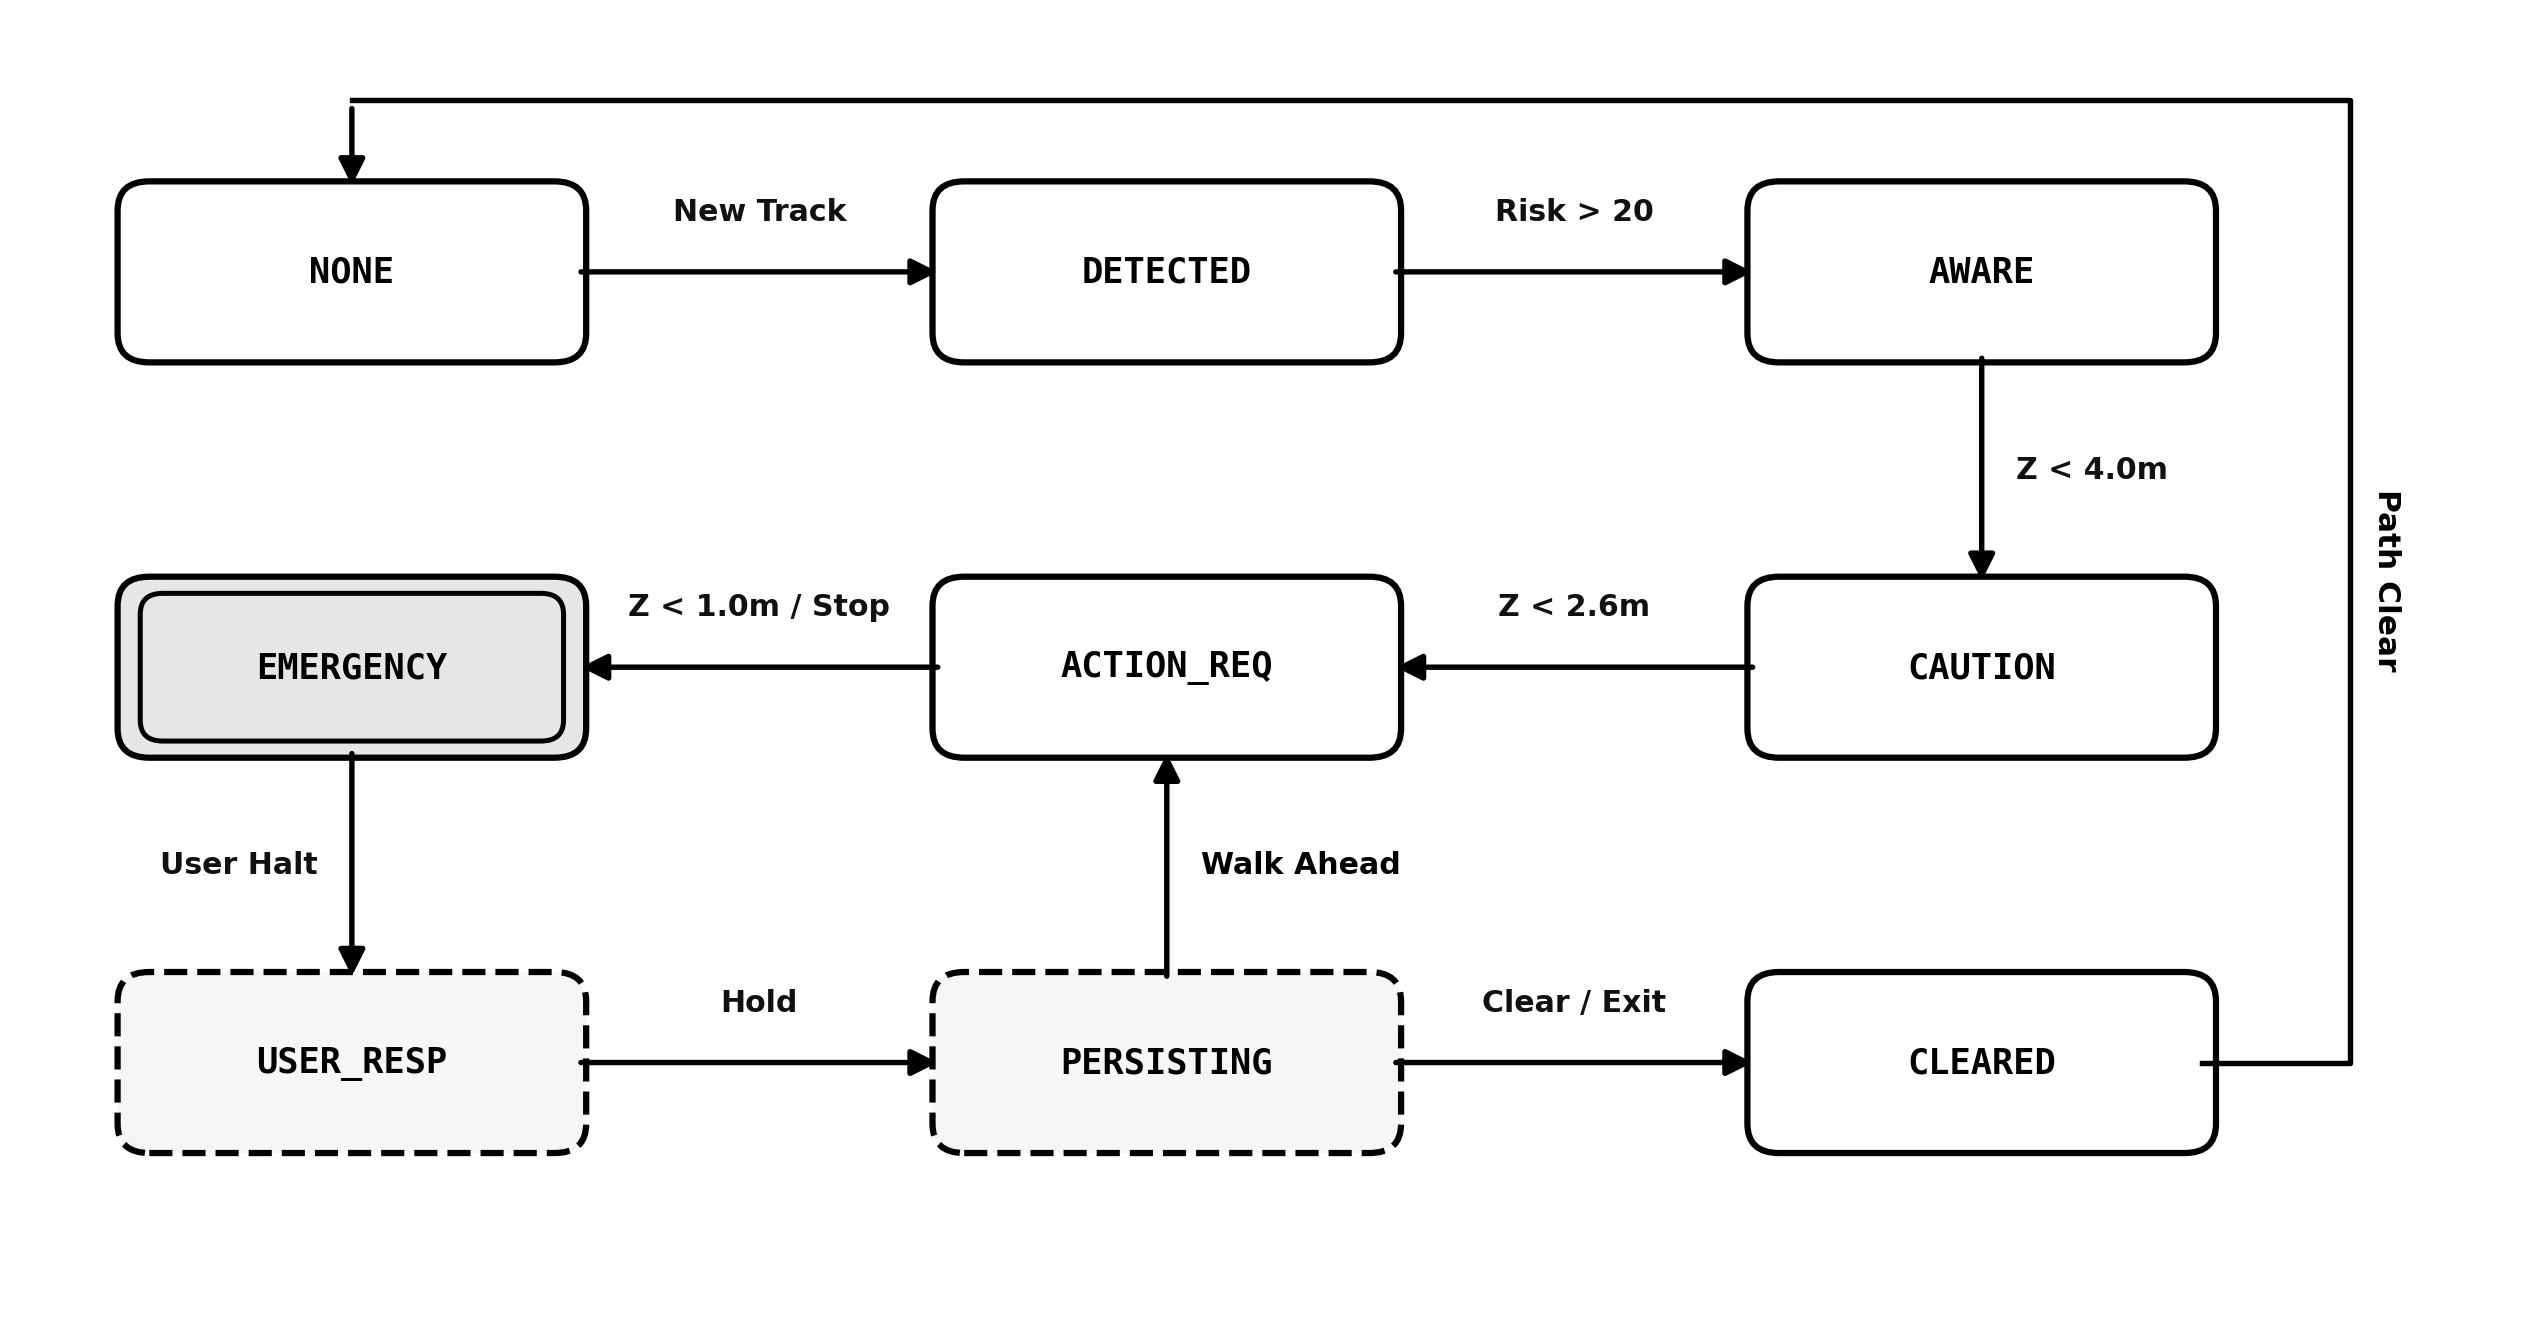
\includegraphics[width=\columnwidth]{figures/fig_hazard_lifecycle.png}
\caption{PRISM 9-state hazard encounter lifecycle state machine (black and white): governs encounter progression from candidate detection to emergency escalation, user halt verification, hold persistence, and hallway clearance.}
\label{fig:hazard_lifecycle}
\end{figure}


\subsection{Collision Risk and Hazard Lifecycle}
\label{sec:impl_collision}
For each confirmed track at relative position $\mathbf{p} = [X, Z]^T$ and velocity $\mathbf{v} = [V_x, V_z]^T$, collision imminence is evaluated analytically using Closest Point of Approach (CPA) and Time-to-Collision (TTC) formulations~\cite{hayward1972characteristics,tam2009review,lee1976theory}:
\begin{align}
t_{\text{CPA}} &= \max\left(0, \, -\frac{\mathbf{p} \cdot \mathbf{v}}{\|\mathbf{v}\|^2}\right), \quad d_{\text{CPA}} = \|\mathbf{p} + \mathbf{v} t_{\text{CPA}}\| \label{eq:cpa} \\
\text{TTC} &= \begin{cases}
-Z / V_z, & \text{if } V_z < -0.10\,\text{m/s} \text{ (approaching)} \\
t_{\text{CPA}}, & \text{if } t_{\text{CPA}} \in [0.1, 4.0]\,\text{s} \text{ and } d_{\text{CPA}} < 0.70\,\text{m} \\
99.0\,\text{s}, & \text{if } V_z > 0.15\,\text{m/s} \text{ (receding)} \\
Z / 1.0, & \text{otherwise (stationary)}
\end{cases} \label{eq:ttc}
\end{align}
Threat confidence $C_{\text{threat}}$ scales from $0.10$ (receding) to $0.95$ (confirmed close in-path). Spatial risk $S \in [0, 100]$ combines distance factor $f_{\text{dist}} = \max(0, 1 - Z/4.5)$, lateral factor $f_{\text{lat}} = \max(0, 1 - |X|/1.2)$, and closing speed multiplier $k_v \in [0.20, 1.30]$, weighted by detection confidence.

\subsubsection{Corridor Arbitration and Decision Policy}
The corridor ($|X| \le 1.2$\,m, $Z < 2.8$\,m) is evaluated for lateral blockage. Navigation actions comprise: \texttt{CONTINUE}, \texttt{SLOW\_DOWN}, \texttt{TURN\_LEFT}, \texttt{TURN\_RIGHT}, and \texttt{EMERGENCY\_STOP}, adapting velocity obstacle principles to indoor walking corridors~\cite{fiorini1998motion,vandenberg2011reciprocal,helbing1995social}. Evasion headings are set to $\theta^* = \pm 0.45$\,rad ($\pm 25.8^\circ$). To prevent steering flapping for centerline obstacles, lateral turn hysteresis imposes a cost barrier $\Delta C = 0.15$. Severe threats ($Z < 1.0$\,m or $S \ge 85.0$) immediately command \texttt{EMERGENCY\_STOP}, bypassing hysteresis.

\subsubsection{Nine-State Hazard Lifecycle}
Hazard encounters progress through a 9-state state machine (Fig.~\ref{fig:hazard_lifecycle}): \texttt{NONE} $\to$ \texttt{DETECTED} $\to$ \texttt{AWARE} $\to$ \texttt{CAUTION} $\to$ \texttt{ACTION\_REQUIRED} $\to$ \texttt{EMERGENCY}. When an emergency stop is issued and the user halts (verified via IMU \texttt{STATIONARY} or $V_z < 0.18$\,m/s), the state transitions to \texttt{USER\_RESPONDING} and holds in \texttt{HAZARD\_PERSISTING}. The hazard clears (\texttt{HAZARD\_CLEARED}) only when distance increases ($Z \ge 1.40$\,m), the entity recedes ($V_z > 0.20$\,m/s), or it exits the corridor ($|X| > 1.25$\,m). Resuming forward walking while the hazard remains close re-escalates to \texttt{EMERGENCY}.

\subsection{Multimodal Warning Generation and Accessibility}
\label{sec:impl_multimodal}
\texttt{WarningMessageGenerator} formats guidance across three complementary channels based on 6 severity tiers, 7 spatial sectors, and 6 distance bands.

\subsubsection{Speech Channel (\texttt{AndroidSpeechChannel})}
Android \texttt{TextToSpeech} generates spoken alerts with audio ducking requested via \texttt{AudioFocusRequest} (\texttt{USAGE\_ASSISTANCE\_NAVIGATION\_GUIDANCE}). Emergency alerts preempt speech via \texttt{QUEUE\_FLUSH}. Cooldown gates limit repetition: 1.0\,s for emergencies, 1.6\,s for directional steering, and 2.5\,s for advisory warnings.

\subsubsection{Spatial Audio Channel (\texttt{AndroidSpatialAudioChannel})}
Directional cues are synthesized via low-latency 44.1\,kHz 16-bit PCM stereo written to \texttt{AudioTrack}, leveraging virtual auditory localization principles~\cite{blauert1997spatial,walker2006navigation}. Linear stereo panning maps spatial direction to channel gains:
\begin{equation}
g_{\text{left}} = \frac{1 - \text{pan}}{2} \cdot V, \quad g_{\text{right}} = \frac{1 + \text{pan}}{2} \cdot V
\label{eq:stereo_panning}
\end{equation}
where $V \in [0, 1]$ represents volume. Chimes use a 20\,ms linear attack and 30\,ms decay over 250\,ms. Emergency cues synthesize an 1100\,Hz dual-harmonic tone. Spatial audio strictly decouples \texttt{HAZARD\_LOCATION} (where an obstacle is) from \texttt{RECOMMENDED\_DIRECTION} (where to steer), preventing conflicting signals. Buffer errors fall back to platform \texttt{ToneGenerator} beeps.

\subsubsection{Haptic Channel and Multisensory Modes}
\texttt{AndroidHapticChannel} delivers \texttt{VibrationEffect} waveform patterns with motor debounce (500\,ms emergency, 1000\,ms regular). The system provides three selectable modes: \texttt{SPEECH\_ONLY}, \texttt{MODE\_A\_SPEECH\_HAPTIC} (speech + vibration), and \texttt{MODE\_B\_SPEECH\_SPATIAL\_HAPTIC} (speech + stereo spatial audio + vibration; default in PRISM-L1.0).
